% ****************************************************************************************
% *****************          PRACTICA: SENSOR DE SISMOS       ****************************
% ****************************************************************************************


% =======================================================
% =======         HEADER FOR DOCUMENT        ============
% =======================================================
    
    % *********   HEADERS AND FOOTERS ********
    \def\ProjectAuthorLink{https://github.com/SoyOscarRH}           %Just to keep it in line
    \def\ProjectNameLink{https://github.com/CompilandoConocimiento} %Just to keep it in line

    % *********   DOCUMENT ITSELF   **************
    \documentclass[12pt, fleqn]{article}                            %Type of docuemtn and size of font and left eq
    \usepackage[margin = 1.2in]{geometry}                           %Margins and Geometry pacakge
    \usepackage[spanish]{babel}                                     %Please use spanish
    \usepackage[utf8]{inputenc}                                     %Please use spanish - UFT
    \usepackage{ifthen}                                             %Allow simple programming
    \usepackage{hyperref}                                           %Create MetaData for a PDF and LINKS!
    \usepackage{pdfpages}                                           %Create MetaData for a PDF and LINKS!
    \hypersetup{pageanchor = false}                                 %Solve 'double page 1' warnings in build
    \setlength{\parindent}{0pt}                                     %Eliminate ugly indentation
    \author{Oscar Andrés Rosas}                                     %Who I am

    % *********   LANGUAJE AND UFT-8   *********
    \usepackage[T1]{fontenc}                                        %Please use spanish
    \usepackage{textcmds}                                           %Allow us to use quoutes
    \usepackage{changepage}                                         %Allow us to use identate paragraphs
    \usepackage{anyfontsize}                                        %All the sizes

    % *********   MATH AND HIS STYLE  *********
    \usepackage{ntheorem, amsmath, amssymb, amsfonts}               %All fucking math, I want all!
    \usepackage{mathrsfs, mathtools, empheq}                        %All fucking math, I want all!
    \usepackage{cancel}                                             %Negate symbol
    \usepackage{centernot}                                          %Allow me to negate a symbol
    \decimalpoint                                                   %Use decimal point

    % *********   GRAPHICS AND IMAGES *********
    \usepackage{graphicx}                                           %Allow to create graphics
    \usepackage{float}                                              %For images
    \usepackage{wrapfig}                                            %Allow to create images
    \graphicspath{ {Graphics/} }                                    %Where are the images :D

    % *********   LISTS AND TABLES ***********
    \usepackage{listings, listingsutf8}                             %We will be using code here
    \usepackage[inline]{enumitem}                                   %We will need to enumarate
    \usepackage{tasks}                                              %Horizontal lists
    \usepackage{longtable}                                          %Lets make tables awesome
    \usepackage{booktabs}                                           %Lets make tables awesome
    \usepackage{tabularx}                                           %Lets make tables awesome
    \usepackage{multirow}                                           %Lets make tables awesome
    \usepackage{multicol}                                           %Create multicolumns

    % *********   HEADERS AND FOOTERS ********
    \usepackage{fancyhdr}                                           %Lets make awesome headers/footers
    \pagestyle{fancy}                                               %Lets make awesome headers/footers
    \setlength{\headheight}{16pt}                                   %Top line
    \setlength{\parskip}{0.5em}                                     %Top line
    \renewcommand{\footrulewidth}{0.5pt}                            %Bottom line

    \lhead{                                                         %Left Header
        \hyperlink{section.\arabic{section}}                        %Make a link to the current chapter
        {\normalsize{\textsc{\nouppercase{\leftmark}}}}             %And fot it put the name
    }

    \rhead{                                                         %Right Header
        \hyperlink{section.\arabic{section}.\arabic{subsection}}    %Make a link to the current chapter
            {\footnotesize{\textsc{\nouppercase{\rightmark}}}}      %And fot it put the name
    }

    \rfoot{\textsc{\small{\hyperref[sec:Index]{Ve al Índice}}}}     %This will always be a footer  

    \fancyfoot[L]{                                                  %Algoritm for a changing footer
        \ifthenelse{\isodd{\value{page}}}                           %IF ODD PAGE:
            {\href{https://compilandoconocimiento.com/nosotros/}    %DO THIS:
                {\footnotesize                                      %Send the page
                    {\textsc{Oscar Andrés Rosas}}}}                 %Send the page
            {\href{https://compilandoconocimiento.com}              %ELSE DO THIS: 
                {\footnotesize                                      %Send the author
                    {\textsc{Laura Andres Morales}}}}               %Send the author
    }
    
    
    
% =======================================================
% ===================   COMMANDS    =====================
% =======================================================

    % =========================================
    % =======   NEW ENVIRONMENTS   ============
    % =========================================
    \newenvironment{Indentation}[1][0.75em]                         %Use: \begin{Inde...}[Num]...\end{Inde...}
        {\begin{adjustwidth}{#1}{}}                                 %If you dont put nothing i will use 0.75 em
        {\end{adjustwidth}}                                         %This indentate a paragraph
    \newenvironment{SmallIndentation}[1][0.75em]                    %Use: The same that we upper one, just 
        {\begin{adjustwidth}{#1}{}\begin{footnotesize}}             %footnotesize size of letter by default
        {\end{footnotesize}\end{adjustwidth}}                       %that's it

    \newenvironment{MultiLineEquation}[1]                           %Use: To create MultiLine equations
        {\begin{equation}\begin{alignedat}{#1}}                     %Use: \begin{Multi..}{Num. de Columnas}
        {\end{alignedat}\end{equation}}                             %And.. that's it!
    \newenvironment{MultiLineEquation*}[1]                          %Use: To create MultiLine equations
        {\begin{equation*}\begin{alignedat}{#1}}                    %Use: \begin{Multi..}{Num. de Columnas}
        {\end{alignedat}\end{equation*}}                            %And.. that's it!
    

    % =========================================
    % == GENERAL TEXT & SYMBOLS ENVIRONMENTS ==
    % =========================================
    
    % =====  TEXT  ======================
    \newcommand \Quote {\qq}                                        %Use: \Quote to use quotes
    \newcommand \Over {\overline}                                   %Use: \Bar to use just for short
    \newcommand \ForceNewLine {$\Space$\\}                          %Use it in theorems for example

    % =====  SPACES  ====================
    \DeclareMathOperator \Space {\quad}                             %Use: \Space for a cool mega space
    \DeclareMathOperator \MegaSpace {\quad \quad}                   %Use: \MegaSpace for a cool mega mega space
    \DeclareMathOperator \MiniSpace {\;}                            %Use: \Space for a cool mini space
    
    % =====  MATH TEXT  =================
    \newcommand \Such {\MiniSpace | \MiniSpace}                     %Use: \Such like in sets
    \newcommand \Also {\MiniSpace \text{y} \MiniSpace}              %Use: \Also so it's look cool
    \newcommand \Remember[1]{\Space\text{\scriptsize{#1}}}          %Use: \Remember so it's look cool
    
    % =====  THEOREMS  ==================
    \newtheorem{Theorem}{Teorema}[section]                          %Use: \begin{Theorem}[Name]\label{Nombre}...
    \newtheorem{Corollary}{Colorario}[Theorem]                      %Use: \begin{Corollary}[Name]\label{Nombre}...
    \newtheorem{Lemma}[Theorem]{Lemma}                              %Use: \begin{Lemma}[Name]\label{Nombre}...
    \newtheorem{Definition}{Definición}[section]                    %Use: \begin{Definition}[Name]\label{Nombre}...
    \theoremstyle{break}                                            %THEOREMS START 1 SPACE AFTER

    % =====  LOGIC  =====================
    \newcommand \lIff {\leftrightarrow}                             %Use: \lIff for logic iff
    \newcommand \lEqual {\MiniSpace \Leftrightarrow \MiniSpace}     %Use: \lEqual for a logic double arrow
    \newcommand \lInfire {\MiniSpace \Rightarrow \MiniSpace}        %Use: \lInfire for a logic infire
    \newcommand \lLongTo {\longrightarrow}                          %Use: \lLongTo for a long arrow

    % =====  FAMOUS SETS  ===============
    \DeclareMathOperator \Naturals     {\mathbb{N}}                 %Use: \Naturals por Notation
    \DeclareMathOperator \Primes       {\mathbb{P}}                 %Use: \Primes por Notation
    \DeclareMathOperator \Integers     {\mathbb{Z}}                 %Use: \Integers por Notation
    \DeclareMathOperator \Racionals    {\mathbb{Q}}                 %Use: \Racionals por Notation
    \DeclareMathOperator \Reals        {\mathbb{R}}                 %Use: \Reals por Notation
    \DeclareMathOperator \Complexs     {\mathbb{C}}                 %Use: \Complex por Notation
    \DeclareMathOperator \GenericField {\mathbb{F}}                 %Use: \GenericField por Notation
    \DeclareMathOperator \VectorSet    {\mathbb{V}}                 %Use: \VectorSet por Notation
    \DeclareMathOperator \SubVectorSet {\mathbb{W}}                 %Use: \SubVectorSet por Notation
    \DeclareMathOperator \Polynomials  {\mathbb{P}}                 %Use: \Polynomials por Notation

    % =====  CONTAINERS   ===============
    \newcommand{\Set}[1]{\left\{ \; #1 \; \right\}}                 %Use: \Set {Info} for INTELLIGENT space 
    \newcommand{\bigSet}[1]{\big\{ \; #1 \; \big\}}                 %Use: \bigSet  {Info} for space 
    \newcommand{\BigSet}[1]{\Big\{ \; #1 \; \Big\}}                 %Use: \BigSet  {Info} for space 
    \newcommand{\biggSet}[1]{\bigg\{ \; #1 \; \bigg\}}              %Use: \biggSet {Info} for space 
    \newcommand{\BiggSet}[1]{\Bigg\{ \; #1 \; \Bigg\}}              %Use: \BiggSet {Info} for space 
    
    \newcommand{\Brackets}[1]{\left[ #1 \right]}                    %Use: \Brackets {Info} for INTELLIGENT space
    \newcommand{\bigBrackets}[1]{\big[ \; #1 \; \big]}              %Use: \bigBrackets  {Info} for space 
    \newcommand{\BigBrackets}[1]{\Big[ \; #1 \; \Big]}              %Use: \BigBrackets  {Info} for space 
    \newcommand{\biggBrackets}[1]{\bigg[ \; #1 \; \bigg]}           %Use: \biggBrackets {Info} for space 
    \newcommand{\BiggBrackets}[1]{\Bigg[ \; #1 \; \Bigg]}           %Use: \BiggBrackets {Info} for space 
    
    \newcommand{\Wrap}[1]{\left( #1 \right)}                        %Use: \Wrap {Info} for INTELLIGENT space
    \newcommand{\bigWrap}[1]{\big( \; #1 \; \big)}                  %Use: \bigBrackets  {Info} for space 
    \newcommand{\BigWrap}[1]{\Big( \; #1 \; \Big)}                  %Use: \BigBrackets  {Info} for space 
    \newcommand{\biggWrap}[1]{\bigg( \; #1 \; \bigg)}               %Use: \biggBrackets {Info} for space 
    \newcommand{\BiggWrap}[1]{\Bigg( \; #1 \; \Bigg)}               %Use: \BiggBrackets {Info} for space 

    % =====  BETTERS MATH COMMANDS   =====
    \newcommand{\pfrac}[2]{\Wrap{\dfrac{#1}{#2}}}                   %Use: Put fractions in parentesis

    % =========================================
    % ====   LINEAL ALGEBRA & VECTORS    ======
    % =========================================

    % ===== UNIT VECTORS  ================
    \newcommand{\hati} {\hat{\imath}}                               %Use: \hati for unit vector    
    \newcommand{\hatj} {\hat{\jmath}}                               %Use: \hatj for unit vector    
    \newcommand{\hatk} {\hat{k}}                                    %Use: \hatk for unit vector

    % ===== MAGNITUDE  ===================
    \newcommand{\abs}[1]{\left\lvert #1 \right\lvert}               %Use: \abs{expression} for |x|
    \newcommand{\Abs}[1]{\left\lVert #1 \right\lVert}               %Use: \Abs{expression} for ||x||
    \newcommand{\Mag}[1]{\left| #1 \right|}                         %Use: \Mag {Info} 
    
    \DeclareMathOperator \LinealTransformation {\mathcal{T}}        %Use: \LinealTransformation for a cool T
    \newcommand{\bVec}[1]{\mathbf{#1}}                              %Use for bold type of vector
    \newcommand{\lVec}[1]{\overrightarrow{#1}}                      %Use for a long arrow over a vector
    \newcommand{\uVec}[1]{\mathbf{\hat{#1}}}                        %Use: Unitary Vector Example: $\uVec{i}

    % ===== ALL FOR DOT PRODUCT  =========
    \makeatletter                                                   %WTF! IS THIS
    \newcommand*\dotP{\mathpalette\dotP@{.5}}                       %Use: \dotP for dot product
    \newcommand*\dotP@[2] {\mathbin {                               %WTF! IS THIS            
        \vcenter{\hbox{\scalebox{#2}{$\m@th#1\bullet$}}}}           %WTF! IS THIS
    }                                                               %WTF! IS THIS
    \makeatother                                                    %WTF! IS THIS

    % === WRAPPERS FOR COLUMN VECTOR ===
    \newcommand{\pVector}[1]                                        %Use: \pVector {Matrix Notation} use parentesis
        { \ensuremath{\begin{pmatrix}#1\end{pmatrix}} }             %Example: \pVector{a\\b\\c} or \pVector{a&b&c} 
    \newcommand{\lVector}[1]                                        %Use: \lVector {Matrix Notation} use a abs 
        { \ensuremath{\begin{vmatrix}#1\end{vmatrix}} }             %Example: \lVector{a\\b\\c} or \lVector{a&b&c} 
    \newcommand{\bVector}[1]                                        %Use: \bVector {Matrix Notation} use a brackets 
        { \ensuremath{\begin{bmatrix}#1\end{bmatrix}} }             %Example: \bVector{a\\b\\c} or \bVector{a&b&c} 
    \newcommand{\Vector}[1]                                         %Use: \Vector {Matrix Notation} no parentesis
        { \ensuremath{\begin{matrix}#1\end{matrix}} }               %Example: \Vector{a\\b\\c} or \Vector{a&b&c}

    % === MAKE MATRIX BETTER  =========
    \makeatletter                                                   %Example: \begin{matrix}[cc|c]
    \renewcommand*\env@matrix[1][*\c@MaxMatrixCols c] {             %WTF! IS THIS
        \hskip -\arraycolsep                                        %WTF! IS THIS
        \let\@ifnextchar\new@ifnextchar                             %WTF! IS THIS
        \array{#1}                                                  %WTF! IS THIS
    }                                                               %WTF! IS THIS
    \makeatother                                                    %WTF! IS THIS

    % =========================================
    % =======   FAMOUS FUNCTIONS   ============
    % =========================================

    % == TRIGONOMETRIC FUNCTIONS  ====
    \newcommand{\Cos}[1] {\cos\Wrap{#1}}                            %Simple wrappers
    \newcommand{\Sin}[1] {\sin\Wrap{#1}}                            %Simple wrappers
    \newcommand{\Tan}[1] {tan\Wrap{#1}}                             %Simple wrappers
    
    \newcommand{\Sec}[1] {sec\Wrap{#1}}                             %Simple wrappers
    \newcommand{\Csc}[1] {csc\Wrap{#1}}                             %Simple wrappers
    \newcommand{\Cot}[1] {cot\Wrap{#1}}                             %Simple wrappers

    % === COMPLEX ANALYSIS TRIG ======
    \newcommand \Cis[1]  {\Cos{#1} + i \Sin{#1}}                    %Use: \Cis for cos(x) + i sin(x)
    \newcommand \pCis[1] {\Wrap{\Cis{#1}}}                          %Use: \pCis for the same with parantesis
    \newcommand \bCis[1] {\Brackets{\Cis{#1}}}                      %Use: \bCis for the same with Brackets


    % =========================================
    % ===========     CALCULUS     ============
    % =========================================

    % ====== TRANSFORMS =============
    \newcommand{\FourierT}[1]{\mathscr{F} \left\{ #1 \right\} }     %Use: \FourierT {Funtion}
    \newcommand{\InvFourierT}[1]{\mathscr{F}^{-1}\left\{#1\right\}} %Use: \InvFourierT {Funtion}

    % ====== DERIVATIVES ============
    \newcommand \MiniDerivate[1][x] {\dfrac{d}{d #1}}               %Use: \MiniDerivate[var] for simple use [var]
    \newcommand \Derivate[2] {\dfrac{d \; #1}{d #2}}                %Use: \Derivate [f(x)][x]
    \newcommand \MiniUpperDerivate[2] {\dfrac{d^{#2}}{d#1^{#2}}}    %Mini Derivate High Orden Derivate -- [x][pow]
    \newcommand \UpperDerivate[3] {\dfrac{d^{#3} \; #1}{d#2^{#3}}}  %Complete High Orden Derivate -- [f(x)][x][pow]
    
    \newcommand \MiniPartial[1][x] {\dfrac{\partial}{\partial #1}}  %Use: \MiniDerivate for simple use [var]
    \newcommand \Partial[2] {\dfrac{\partial \; #1}{\partial #2}}   %Complete Partial Derivate -- [f(x)][x]
    \newcommand \MiniUpperPartial[2]                                %Mini Derivate High Orden Derivate -- [x][pow] 
        {\dfrac{\partial^{#2}}{\partial #1^{#2}}}                   %Mini Derivate High Orden Derivate
    \newcommand \UpperPartial[3]                                    %Complete High Orden Derivate -- [f(x)][x][pow]
        {\dfrac{\partial^{#3} \; #1}{\partial#2^{#3}}}              %Use: \UpperDerivate for simple use

    \DeclareMathOperator \Evaluate  {\Big|}                         %Use: \Evaluate por Notation

    % =========================================
    % ========    GENERAL STYLE     ===========
    % =========================================
    
    % =====  COLORS ==================
    \definecolor{RedMD}{HTML}{F44336}                               %Use: Color :D        
    \definecolor{Red100MD}{HTML}{FFCDD2}                            %Use: Color :D        
    \definecolor{Red200MD}{HTML}{EF9A9A}                            %Use: Color :D        
    \definecolor{Red300MD}{HTML}{E57373}                            %Use: Color :D        
    \definecolor{Red700MD}{HTML}{D32F2F}                            %Use: Color :D 

    \definecolor{PurpleMD}{HTML}{9C27B0}                            %Use: Color :D        
    \definecolor{Purple100MD}{HTML}{E1BEE7}                         %Use: Color :D        
    \definecolor{Purple200MD}{HTML}{EF9A9A}                         %Use: Color :D        
    \definecolor{Purple300MD}{HTML}{BA68C8}                         %Use: Color :D        
    \definecolor{Purple700MD}{HTML}{7B1FA2}                         %Use: Color :D 

    \definecolor{IndigoMD}{HTML}{3F51B5}                            %Use: Color :D        
    \definecolor{Indigo100MD}{HTML}{C5CAE9}                         %Use: Color :D        
    \definecolor{Indigo200MD}{HTML}{9FA8DA}                         %Use: Color :D        
    \definecolor{Indigo300MD}{HTML}{7986CB}                         %Use: Color :D        
    \definecolor{Indigo700MD}{HTML}{303F9F}                         %Use: Color :D 

    \definecolor{BlueMD}{HTML}{2196F3}                              %Use: Color :D        
    \definecolor{Blue100MD}{HTML}{BBDEFB}                           %Use: Color :D        
    \definecolor{Blue200MD}{HTML}{90CAF9}                           %Use: Color :D        
    \definecolor{Blue300MD}{HTML}{64B5F6}                           %Use: Color :D        
    \definecolor{Blue700MD}{HTML}{1976D2}                           %Use: Color :D        
    \definecolor{Blue900MD}{HTML}{0D47A1}                           %Use: Color :D  

    \definecolor{CyanMD}{HTML}{00BCD4}                              %Use: Color :D        
    \definecolor{Cyan100MD}{HTML}{B2EBF2}                           %Use: Color :D        
    \definecolor{Cyan200MD}{HTML}{80DEEA}                           %Use: Color :D        
    \definecolor{Cyan300MD}{HTML}{4DD0E1}                           %Use: Color :D        
    \definecolor{Cyan700MD}{HTML}{0097A7}                           %Use: Color :D        
    \definecolor{Cyan900MD}{HTML}{006064}                           %Use: Color :D 

    \definecolor{TealMD}{HTML}{009688}                              %Use: Color :D        
    \definecolor{Teal100MD}{HTML}{B2DFDB}                           %Use: Color :D        
    \definecolor{Teal200MD}{HTML}{80CBC4}                           %Use: Color :D        
    \definecolor{Teal300MD}{HTML}{4DB6AC}                           %Use: Color :D        
    \definecolor{Teal700MD}{HTML}{00796B}                           %Use: Color :D        
    \definecolor{Teal900MD}{HTML}{004D40}                           %Use: Color :D 

    \definecolor{GreenMD}{HTML}{4CAF50}                             %Use: Color :D        
    \definecolor{Green100MD}{HTML}{C8E6C9}                          %Use: Color :D        
    \definecolor{Green200MD}{HTML}{A5D6A7}                          %Use: Color :D        
    \definecolor{Green300MD}{HTML}{81C784}                          %Use: Color :D        
    \definecolor{Green700MD}{HTML}{388E3C}                          %Use: Color :D        
    \definecolor{Green900MD}{HTML}{1B5E20}                          %Use: Color :D

    \definecolor{AmberMD}{HTML}{FFC107}                             %Use: Color :D        
    \definecolor{Amber100MD}{HTML}{FFECB3}                          %Use: Color :D        
    \definecolor{Amber200MD}{HTML}{FFE082}                          %Use: Color :D        
    \definecolor{Amber300MD}{HTML}{FFD54F}                          %Use: Color :D        
    \definecolor{Amber700MD}{HTML}{FFA000}                          %Use: Color :D        
    \definecolor{Amber900MD}{HTML}{FF6F00}                          %Use: Color :D

    \definecolor{BlueGreyMD}{HTML}{607D8B}                          %Use: Color :D        
    \definecolor{BlueGrey100MD}{HTML}{CFD8DC}                       %Use: Color :D        
    \definecolor{BlueGrey200MD}{HTML}{B0BEC5}                       %Use: Color :D        
    \definecolor{BlueGrey300MD}{HTML}{90A4AE}                       %Use: Color :D        
    \definecolor{BlueGrey700MD}{HTML}{455A64}                       %Use: Color :D        
    \definecolor{BlueGrey900MD}{HTML}{263238}                       %Use: Color :D        

    \definecolor{DeepPurpleMD}{HTML}{673AB7}                        %Use: Color :D

    \newcommand{\Color}[2]{\textcolor{#1}{#2}}                      %Simple color environment
    \newenvironment{ColorText}[1]                                   %Use: \begin{ColorText}
        { \leavevmode\color{#1}\ignorespaces }                      %That's is!

    % =====  CODE EDITOR =============
    \lstdefinestyle{CompilandoStyle} {                              %This is Code Style
        backgroundcolor     = \color{BlueGrey900MD},                %Background Color  
        basicstyle          = \tiny\color{white},                   %Style of text
        commentstyle        = \color{BlueGrey200MD},                %Comment style
        stringstyle         = \color{Green300MD},                   %String style
        keywordstyle        = \color{Blue300MD},                    %keywords style
        numberstyle         = \tiny\color{TealMD},                  %Size of a number
        frame               = shadowbox,                            %Adds a frame around the code
        breakatwhitespace   = true,                                 %Style   
        breaklines          = true,                                 %Style   
        showstringspaces    = false,                                %Hate those spaces                  
        breaklines          = true,                                 %Style                   
        keepspaces          = true,                                 %Style                   
        numbers             = left,                                 %Style                   
        numbersep           = 10pt,                                 %Style 
        xleftmargin         = \parindent,                           %Style 
        tabsize             = 4,                                    %Style
        inputencoding       = utf8/latin1                           %Allow me to use special chars
    }
 
    \lstset{style = CompilandoStyle}                                %Use this style







% =====================================================
% ============        COVER PAGE       ================
% =====================================================
\begin{document}
\begin{titlepage}
    
    % ============ TITLE PAGE STYLE  ================
    \definecolor{TitlePageColor}{cmyk}{1,.60,0,.40}                 %Simple colors
    \definecolor{ColorSubtext}{cmyk}{1,.50,0,.10}                   %Simple colors
    \newgeometry{left=0.20\textwidth}                               %Defines an Offset
    \pagecolor{TitlePageColor}                                      %Make it this Color to page
    \color{white}                                                   %General things should be white

    % ===== MAKE SOME SPACE =========
    \vspace                                                         %Give some space
    \baselineskip                                                   %But we need this to up command

    % ============ NAME OF THE PROJECT  ============
    \makebox[0pt][l]{\rule{1.3\textwidth}{3pt}}                     %Make a cool line
    
    \href{https://compilandoconocimiento.com}                       %Link to project
    {\textbf{\textsc{\Huge ESCOM - IPN}}}\\[2.7cm]                  %Name of project   

    % ============ NAME OF THE BOOK  ===============
    \href{\ProjectNameLink/LibroAnalisisDeAlgoritmos}               %Link to Author
    {\fontsize{35}{40}                                              %Size of the book
        \selectfont
        \textbf{Proyecto: \\Sensor Sísmico - El Pequeño Molesto}}\\[0.5cm]               %Name of the book
    \textcolor{ColorSubtext}                                        %Color or the topic
        {\textsc{\LARGE Instrumentación}}\\[0.5cm]                  %Name of the general theme
    
    
    \vfill                                                          %Fill the space
    
    % ============ NAME OF THE AUTHOR  =============
    \href{\ProjectAuthorLink}                                       %Link to Author
    {\LARGE 
    \textsf{Oscar Andrés Rosas Hernandez y Laura Andres Morales}}   %Author

    % ===== MAKE SOME SPACE =========
    \vspace                                                         %Give some space
    \baselineskip                                                   %But we need this to up command
    
    {\large \textsf{Realizada 14 de Marzo 2018}}                    %Date
    
    {\large \textsf{Entregada 15 de Marzo 2018}}                    %Date

\end{titlepage}


% =====================================================
% ==========      RESTORE TO DOCUMENT      ============
% =====================================================
\restoregeometry                                                    %Restores the geometry
\nopagecolor                                                        %Use to restore the color to white




% =====================================================
% ========                INDICE              =========
% =====================================================
\tableofcontents{}
\label{sec:Index}

\clearpage



% ===============================================================================
% ===================          INTRODUCCIÓN                ======================
% ===============================================================================
\section{Introducción: Sismos}

    Anualmente los sismógrafos registran aproximadamente 20.000 sismos en todo el
    planeta. Los expertos y científicos están completamente de acuerdo: millones de
    persones en las grandes ciudades con riesgos de sismicidad, están amenazadas en un
    futuro no muy lejano por terremotos, sobre los cuales no están preparados o no en la
    forma adecuada.
    A pesar de que las normativas de construcción cada vez han sido más rígidas y estrictas,
    miles de personas han perecido en edificaciones que han cedido o por el fuego que en
    ellos se ha desatado debido a las tuberías de gas y los cables eléctricos de la fuente de
    alimentación que se han destruido. 


    Los terremotos son sacudidas del terreno con limitaciones en el tiempo, las mismas
    que se propagan en diferentes amplitudes de ondas desde su origen (epicentro) en todos
    los sentidos.


    % ==============================================================
    % =================      ONDAS PRIMARIAS      ==================
    % ==============================================================
    \subsection{Ondas Primarias}

        La Onda Primaria de un terremoto, para el ser humano no es perceptible, se expande
        desde el punto de origen (Epicentro) del terremoto con mayor rapidez, antes de la
        llegada de la destructora Onda Secundaria.

        Con ello, la Onda Primaria alcanzará siempre como primer punto, el lugar en el cual se
        encuentra instalado el sistema con sensores.


    % ==============================================================
    % =================      ONDAS SECUNDARIAS    ==================
    % ==============================================================
    \subsection{Ondas Secundarias}

        La Onda Secundaria viene inevitablemente detrás de la Onda primaria. Mientras más
        lejos se encuentre el lugar en el cual se origina el terremoto (epicentro) al lugar en el
        cual se encuentran instalados los sensores, mayor será el tiempo entre la llegada de la
        Onda Primaria con respecto a la Onda Secundaria. El tiempo que queda entre la llegada
        de la Onda Primaria y la llegada de la Onda Secundaria es el tiempo de alerta previa y
        acción que tiene el ser humano y su entorno.

        Entre la Onda Primaria y la Onda Secundaria de un terremoto existen dependencias de
        naturaleza física. La característica de la Onda Primaria permite sacar conclusiones de la
        Onda Secundaria posterior que viene con mayor fuerza y su esperado poder destructivo.





% ===============================================================================
% ===================          INTRODUCCIÓN                ======================
% ===============================================================================
\clearpage
\section{Introducción: Sensores Sismicos}

    \begin{wrapfigure}{r}{0.25\textwidth}
        \centering
        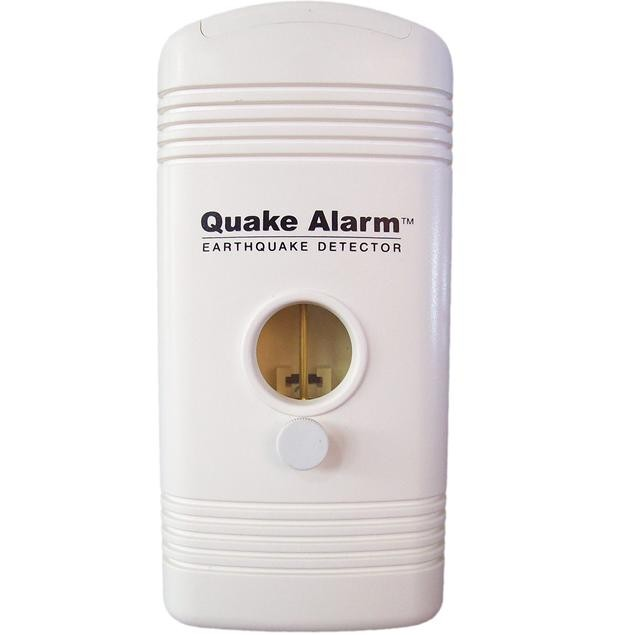
\includegraphics[width=0.45\textwidth]{Quake}
    \end{wrapfigure}

    Usamos el sensor dentro del Quake Alarm como base para nuestro sensor, este es 
    una alarma comercial que funciona independientemente de un sistema de alimentación
    gracias a una bateria.

    Este se coloca sobre una superficie y nos alerta con una alarma sonora sobre posibles movimientos
    teluricos, además de poder modificar su sensibilidad para poder tener mejor control sobre el mismo
    sensor.

    Está diseñado para proporcionar una advertencia instantánea de la actividad sísmica mediante la detección
    de la onda "p" (onda de compresión) de un terremoto, que viaja más rápido que la onda más destructiva "s"
    (onda de corte). 


    % ==============================================================
    % ========     FUNCIONAMIENTO FISICO          ==================
    % ==============================================================
    \subsection{Funcionamiento}

        La base del funcionamiento de este circuito es bastante sencillo una vez que se abre, se usa
        un péndulo invertido con una masa de metal en la parte superior, esto no da una solución a los
        problemas de sensibilidad.

        En la aprte inferior del péndulo se encuentra una arilla de metal que hace de conductor con la parte
        principal activando el sensor cuando es que ambas piezas métalicas se tocan, esta puede subir o bajar
        gracias a una pequeña perilla, con lo que los movimientos necesarios para que el sensor se active
        pueden variar, desde en la parte superior con una sensibilidad máxima, pues un pequeño movimiento
        hará que la barra vibra fuertemente y con ello se active, mientras que en la parte inferior tendrá que
        ser una actividad de mucho mayor magnitud para causar que el sensor se active.

        Una vez que las piezas se tocan estas cierran un circuito de control, es decir, a efectos
        practicos este sensor funciona como un simple switch que al momento de recibir un movimiento
        cierra en switch.

        Este funciona con una pila de 9v, lo cual le permite su portabilidad, además gracias a que literalmente
        no hay continuidad cuando el sensor esta apagado entonces la vida útil del funcionamiento del sensor es
        practicamente la misma que la vida útil de las baterias en reposo.



% ===============================================================================
% ===================          DESARROLLO                  ======================
% ===============================================================================
\clearpage
\section{Desarrollo}


    % ==============================================================
    % =================      DIAGRAMAS            ==================
    % ==============================================================
    \subsection{Diagramas}

        Veamos que nuestro circuito puede ser descrito con el siguiente diagrama:
        \begin{figure}[h]
            \centering
            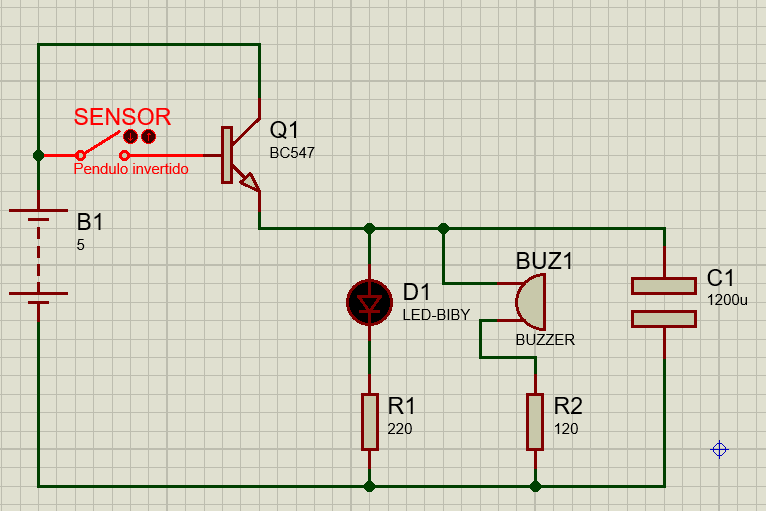
\includegraphics[width=0.85\textwidth]{PequenoMolesto}
        \end{figure}

        Este lo podemos dividir basicamente en 2 partes:
        \begin{itemize}
            \item 
                \textbf{Circuito Sensor}

                Consta de 2 partes, es básicamente un switch, se coloca el pendulo como una parte del mismo, y una base que será la segunda.
                
                Usamos un candado como peso principal y un palo de paleta para el pendulo, esto lo recubrimos de cable y logramos que condujera hasta la base del mismo, después la base fue un anillo recubierto de cable, esots elementos se calibraron con una sensibilidad alta, una vez que estuvimos contentos con la sensibilidad pasamos a la etapa del circuito.

   
            \item 
                \textbf{Circuito Control}

                 Como se mencionó es un switch y para evitar pulsos bajos o con poco amperaje lo que se hizo fue colocar un transistor NPN de manera que una vez que recibiera el pulso lo dejara pasar por el colector y el emisor.
                 
                 Para nuestra aplicación para evitr que el pulso se perdiera rápido usamos un capacitor, eso nos dio un rango mayor de pulsos.


            \item 
                \textbf{Aplicación}
                   Colocamos un buzzer Pequeño y Molesto pues su frecuencia es aguda y estresante, además que cambia con respecto a la intensidad del pulso que recibe, adicional colocamos un led ultra brillante.


        \end{itemize}


    % ==============================================================
    % =================      CIRCUITO REAL        ==================
    % ==============================================================
    \subsection{Circuito Real}

        Veamos que nuestro circuito fue construido de la siguiente manera:
        \begin{figure}[h]
            \centering
            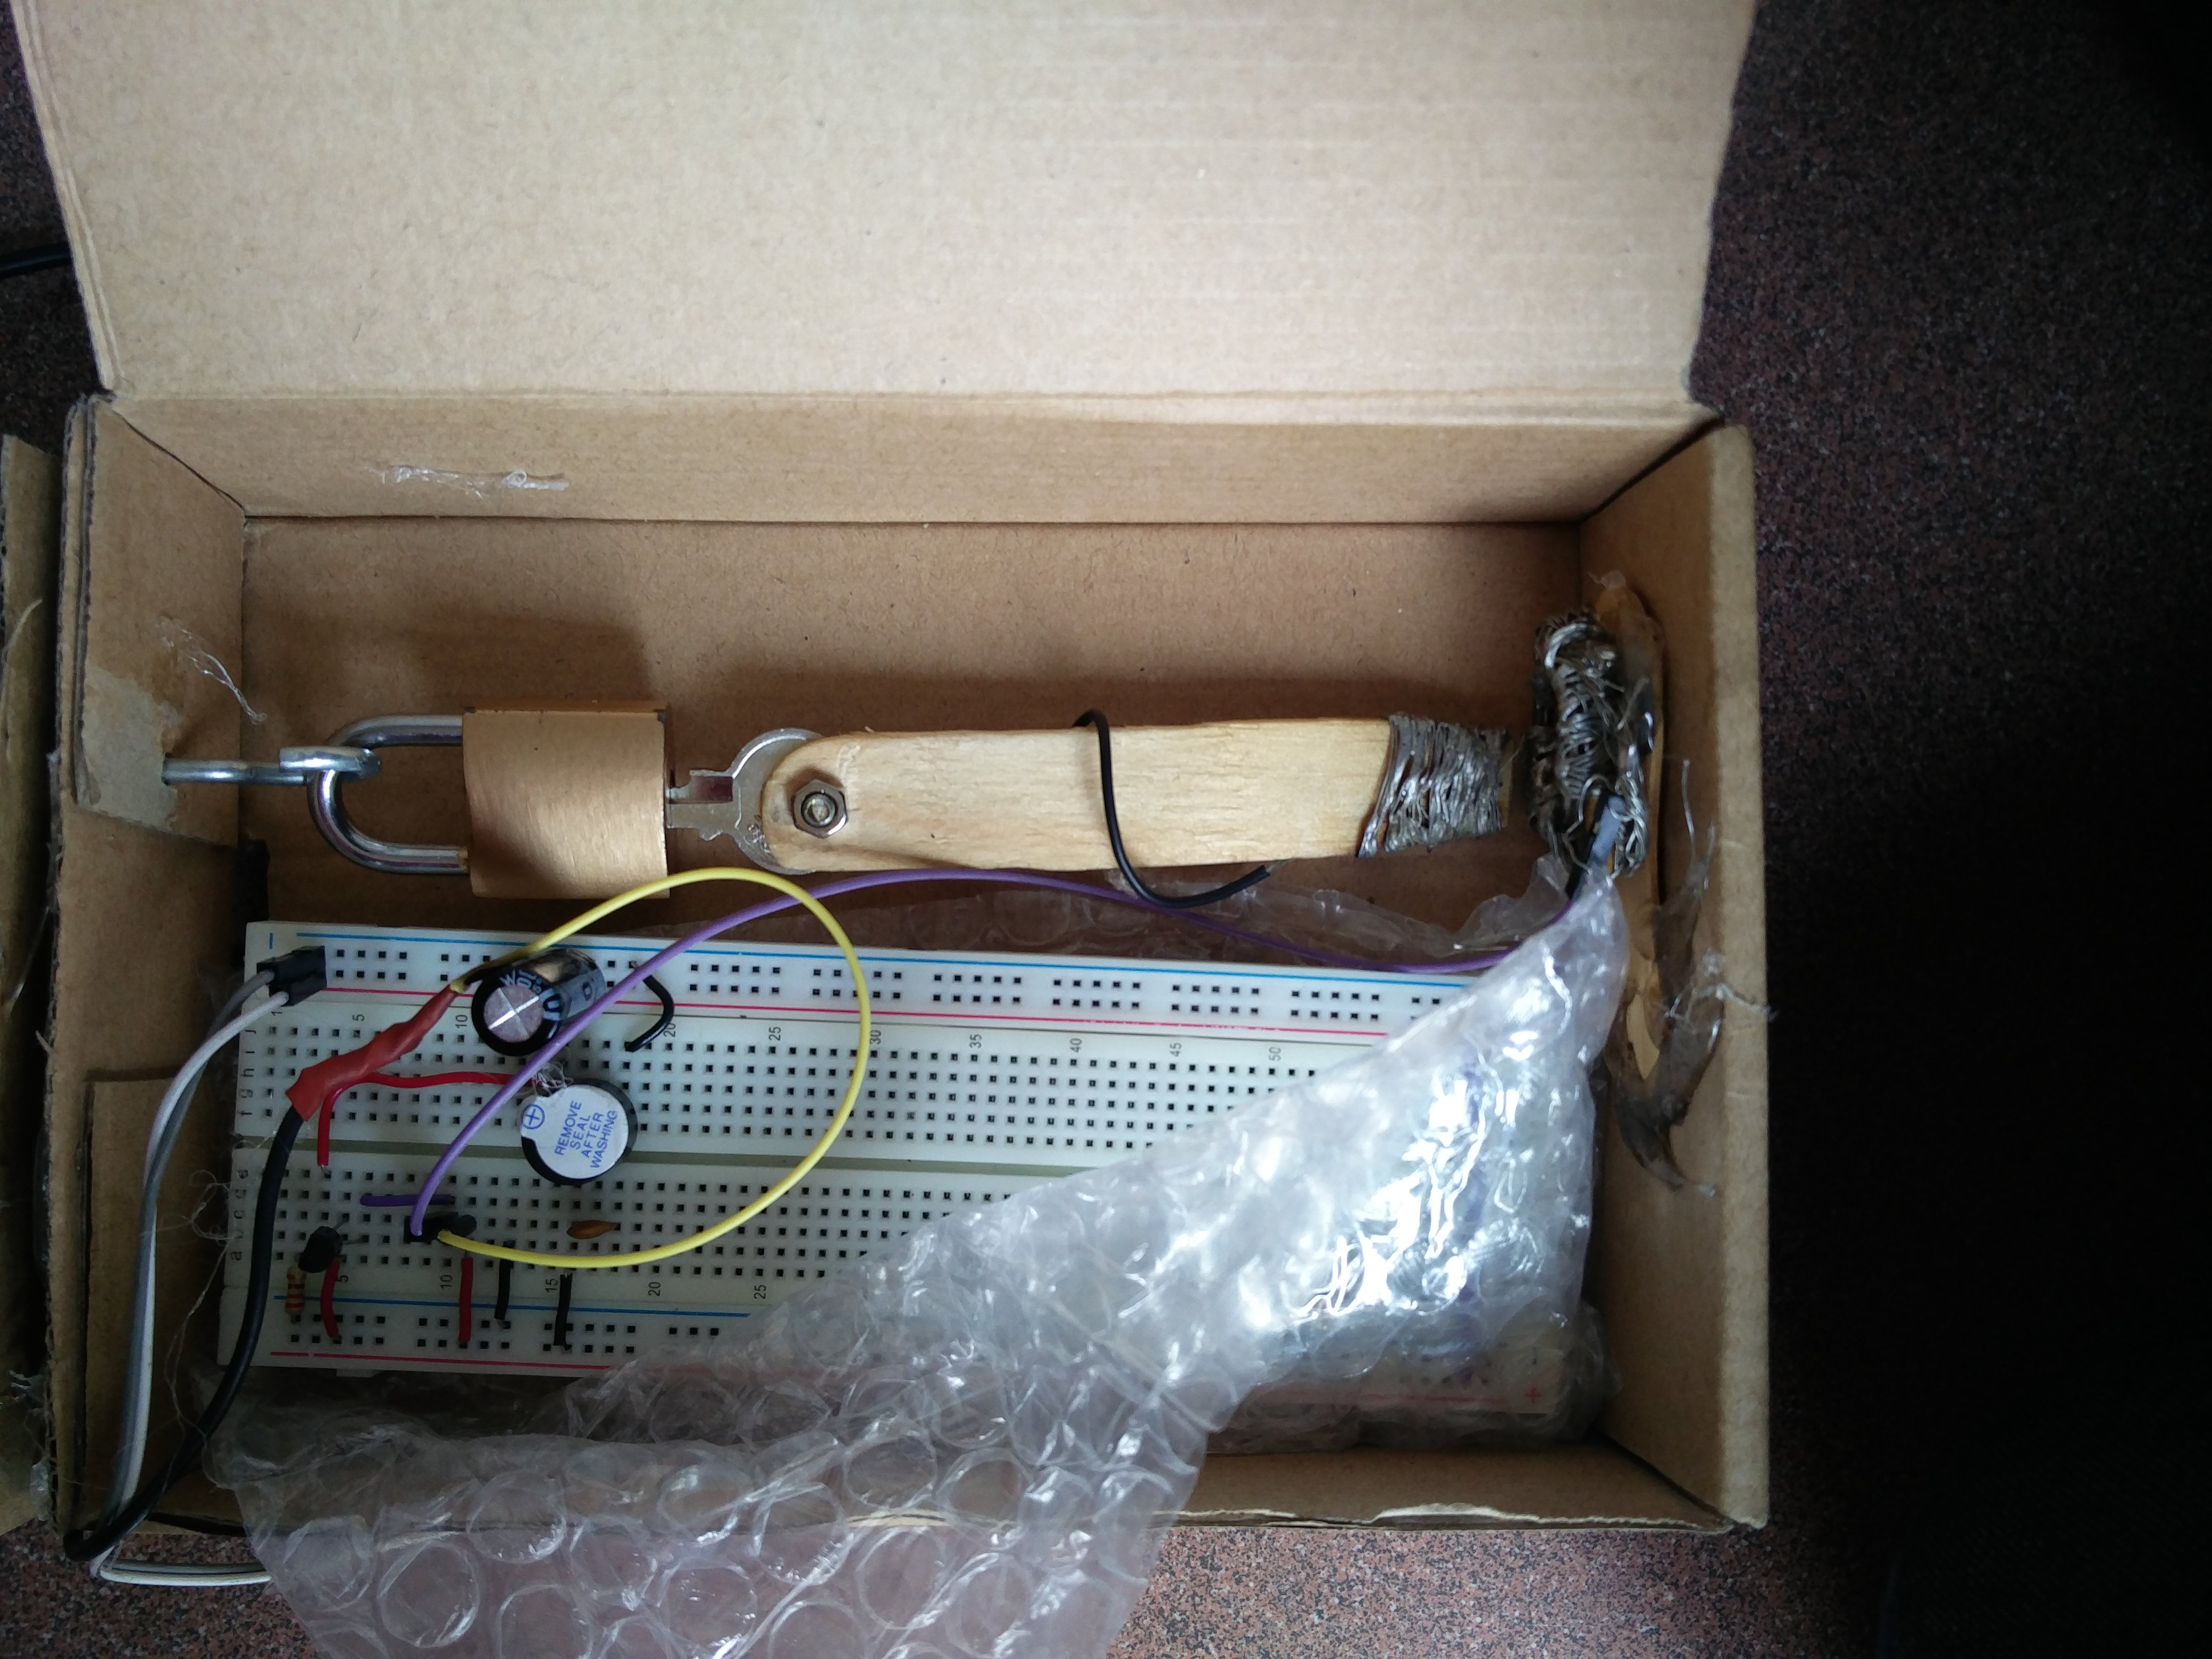
\includegraphics[width=0.85\textwidth]{Real2}
        \end{figure}
        
        \begin{figure}[h]
            \centering
            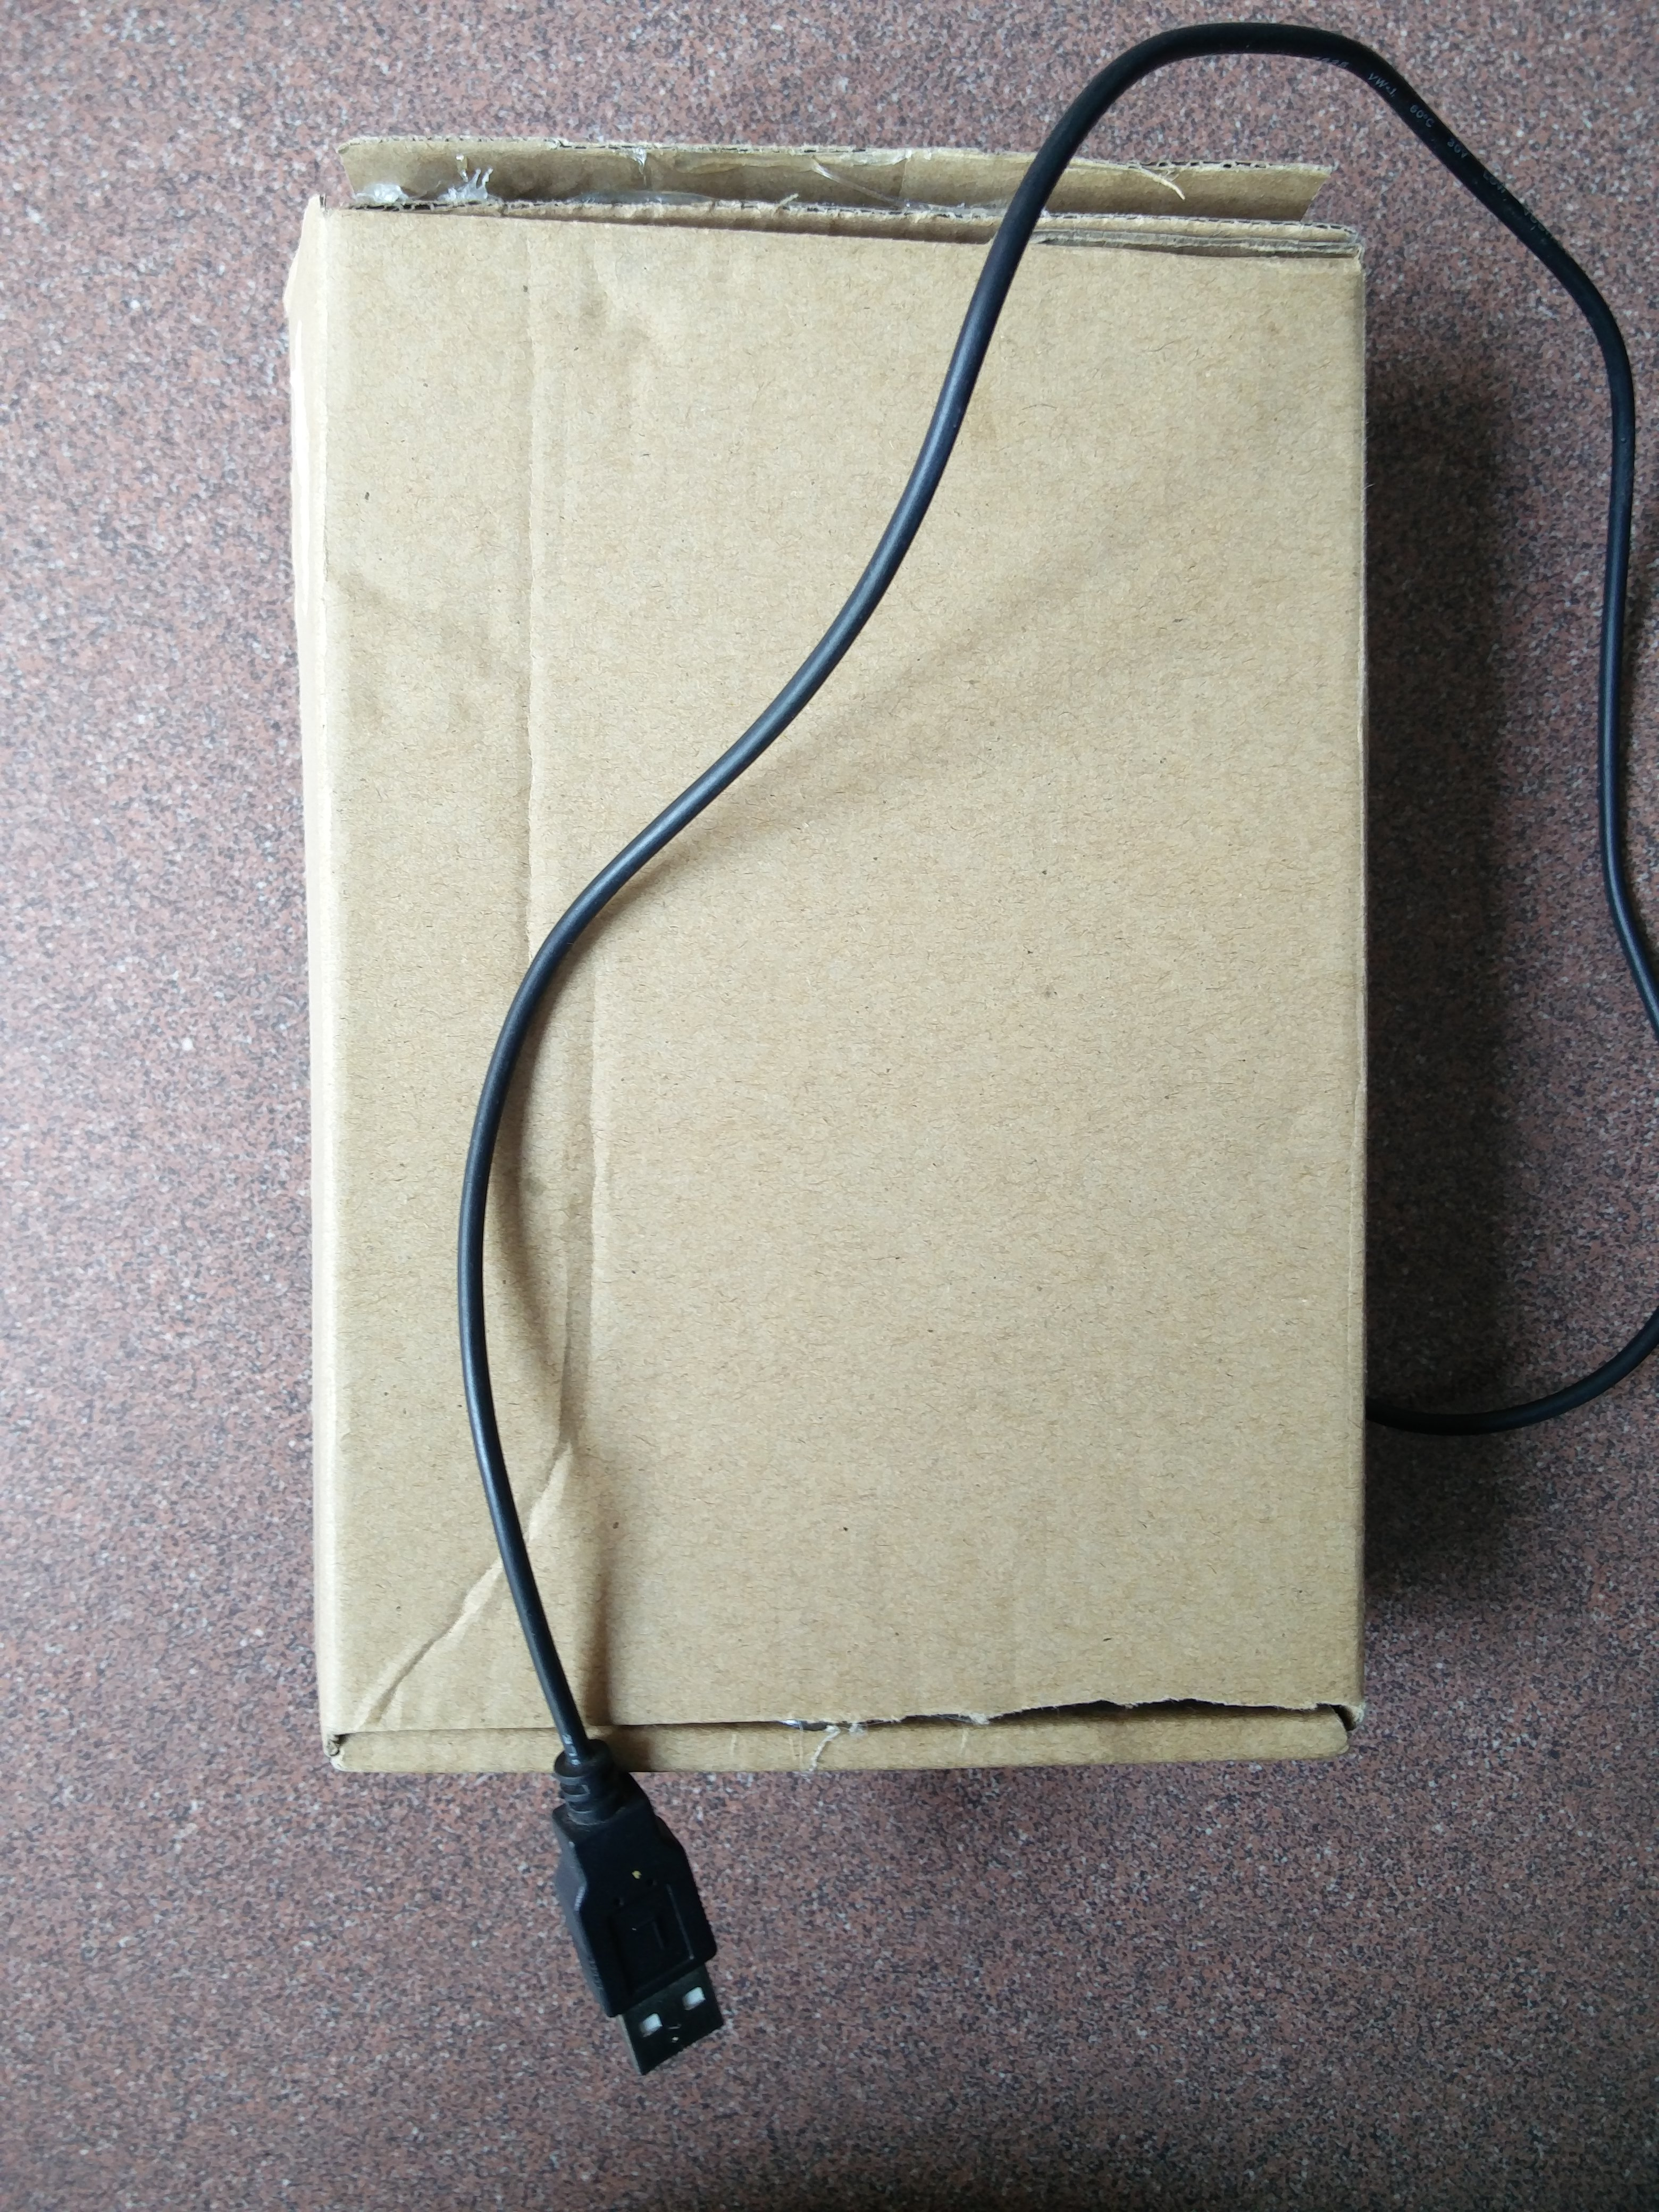
\includegraphics[width=0.35\textwidth]{Real1}
        \end{figure}


    % ==============================================================
    % =================      MEDICIONES           ==================
    % ==============================================================
    \subsection{Experiencias del Circuito Real}

        Nosotros no usamos un pendulo invertido, sino un pendulo concenvional, en el que el punto que no se
        mueve, estacionario esta en la parte superior, por lo tanto mientras mas abajo estuviera nuestro
        anillo conductor más sensible será nuestro aparato, para poder tener una gran sensibilidad decidimos tener
        fijo el anillo en la parte inferior, con ello logramos una sensibilidad impresionante, pero también se agravio
        mucho más el problema del nivelado, pues al colocar el sensor en una superficie desnivelada nos daba un
        falso positivo.

        Por otro lado, debido a que los sismos están caracterizados como un grupo de pequeñas oscilasciones decidimos
        conectar un capacitor de 2,200 $\mu F$ con lo que pudimos pasar de una señal intermitente a una señal continua
        en el caso de oscilasciones rápidas características de un temblor.


        Además para nuestro diseño decidimos usar un cable USB modificado, tomando solo nuestro circuito los 2
        pines de alimentación, con lo que nuestros sistema podría instalarse con la facilidad con la que conectamos
        nuestro celular a la mesa de noche o nuestra licuadora en la cocina, es decir una conexión estable.

        De igual manera, gracias a usar USB podemos conectarlo por ejemplo a una batería portatil y ya que al
        igual que nuestro circuito de refencia este no gaste energía en reposo podría quedar activo sin cables
        y siendo alimentado solo por una batería portátil.

    % ==============================================================
    % =================      MEDICIONES           ==================
    % ==============================================================
    \subsection{Mediciones}

        En este caso decidimos no añadimos mediciones porque nuestro sensor solo tiene 2 posibles
        estados, por lo que todas las mediciones sería o bien $5v$ o $0v$.

    % ==============================================================
    % =============     CONCLUSIONES      ==========================
    % ==============================================================
    \clearpage
    \subsection{Conclusiones} 

        Gracias a este pequeño proyecto pudimos comprobar la facilidad con la que podemos 
        crear un sensor sismico usando la variación en las vibraciones y como un doble péndulo
        puede ayudarnos con la sensibilidad a la hora de crear nuestro sensor sísmico.

        Comprobamos que el principal problema de este clase de diseños es que su funcionamiento solo es optimo
        si es que se colocan sobre una superficie que este complemente plana, de otro modo
        es muy fácil que la sensibilidad llene o bien a que no se detenten movimiento o bien a que
        se detecten falsos positivos.


    % ==============================================================
    % ==========    APLICACION TENTATIVA     =======================
    % ==============================================================
    \subsection{Aplicación Tentativa} 

        La aplicación más obvia es conectar el sensor a una bocina como por ejemplo nuestro
        sistema de refencia y con este alerta a las personas
        del peligro, pero no es lo único para lo que se puede usar, pues que ya se puede identificar el sismo,
        podemos también usar la salida de nuestro sistema de acondionamiento para poder conectar a varios
        relays es decir que al mismo tiempo que mandamos nuestra señal de alarma
        también de forma automática accionar todos los elementos eléctricos y electrónicos que han sido 
        programados con el sensor.

        Un posible diagrama de esta aplicación puede ser:

        \begin{figure}[h]
            \centering
            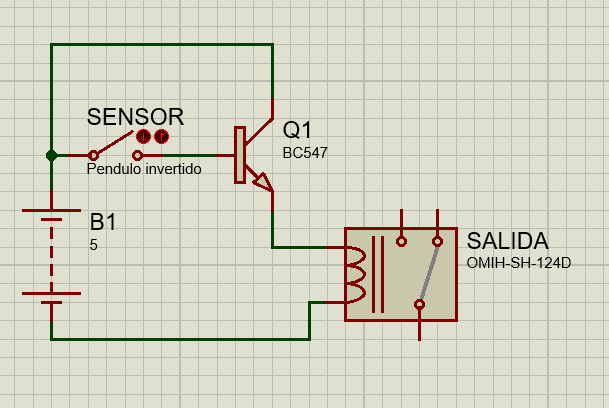
\includegraphics[width=0.85\textwidth]{Usos}
        \end{figure}
        Así se puede por ejemplo:
        \begin{itemize}
            \item Desconectar suministros de gas centralizado y energía eléctrica
            \item Bloquear el suministro de agua potable
            \item Encender generadores de emergencia
            \item Controlar los ascensores
            \item Abrir puertas y sistemas de seguridad
            \item Activar señales sonoras mucho más intensas
            \item Activar señalizaciones en los puentes y entradas a túneles
            \item Activación de computadoras para respaldar información automáticamente
        \end{itemize}









\end{document}